\normaltrue \difficilefalse \tdifficilefalse
\correctiontrue

%\UPSTIidClasse{11} % 11 sup, 12 spé
\renewcommand{\UPSTIidClasse}{12}

\exer{Cheville robot NAO$\star$ \label{C2:06:25}}
\setcounter{numques}{0}
\UPSTIcompetence[2]{A3-05}
\UPSTIcompetence[2]{C2-06}
\index{Compétence C2-06}
\index{Train d'engrenages simple}
\index{Cheville robot NAO}
\ifcorrection
\else
\textbf{Pas de corrigé pour cet exercice.}
\fi

\ifprof
\else
On s'intéresse ici à la cheville NAO. On cherche à savoir si, à partir du moteur retenu par le constructeur, la chaîne de transmission de puissance permet de vérifier les exigences suivantes : 
\begin{itemize}
\item exigence 1.1.1.1 : la vitesse de roulis doit être inférieure à \SI{42}{tr/min};
\item exigence 1.1.1.2 : la vitesse de tangage doit être inférieure à \SI{60}{tr/min}.
\end{itemize}
%\begin{center}
%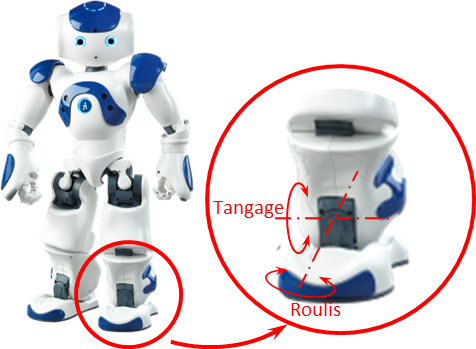
\includegraphics[width=.7\linewidth]{25_01}
%\end{center}


La fréquence de rotation des moteurs permettant chacun des deux mouvements est de \SI{8300}{tr/min}.

Pour la chaîne de transmission de tangage on donne  le nombre de dents et le module de chaque roue dentée : 
\begin{itemize}
\item pignon moteur : $Z_m=20$, $M_m=0,3$;
\item grand pignon 1 : $Z_1 = 80$, $M_1=0,3$;
\item petit pignon 1 : $Z_1' = 25$, $M_1'=0,4$;
\item grand pignon 2 : $Z_2 = 47$, $M_2=0,4$;
\item petit pignon 2 : $Z_2' = 12$, $M_2'=0,4$;
\item grand pignon 3 : $Z_3 = 58$, $M_3=0,4$;
\item petit pignon 3 : $Z_3' = 10$, $M_3'=0,7$;
\item roue de sortie : $Z_T = 36$, $M_T=0,7$.
\end{itemize}

\begin{center}
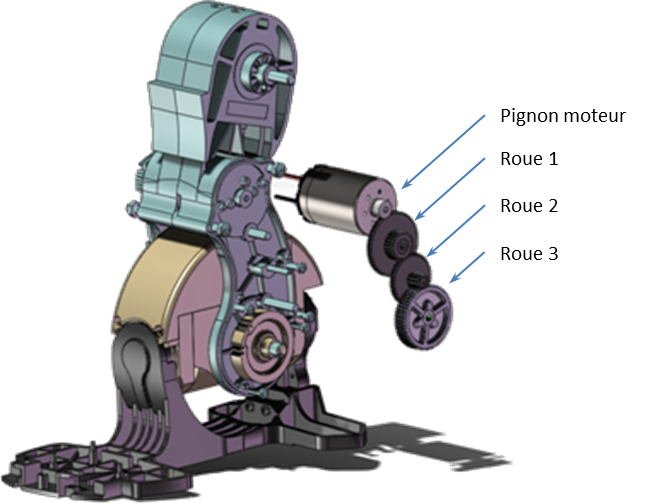
\includegraphics[width=.8\linewidth]{25_02}
\end{center}

Pour la chaîne de transmission du roulis on donne le nombre de dents et le module de chaque roue dentée : 
\begin{itemize}
\item pignon moteur : $Z_m=13$, $M_m=0,3$;
\item grand pignon 1 : $Z_1 = 80$, $M_1=0,3$;
\item petit pignon 1 : $Z_1' = 25$, $M_1'=0,4$;
\item grand pignon 2 : $Z_2 = 47$, $M_2=0,4$;
\item petit pignon 2 : $Z_2' = 12$, $M_2'=0,4$;
\item grand pignon 3 : $Z_3 = 58$, $M_3=0,4$;
\item petit pignon 3 : $Z_3' = 10$, $M_3'=0,7$;
\item roue de sortie 3 : $Z_R = 36$, $M_R=0,7$.
\end{itemize}



\begin{center}
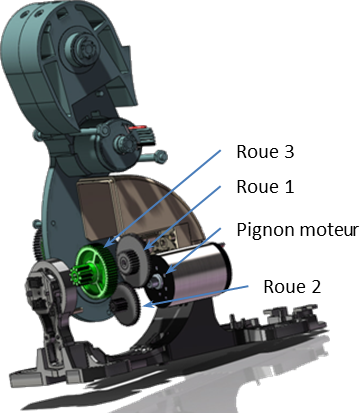
\includegraphics[width=.7\linewidth]{25_03}
\end{center}
\fi



\question{Quels doivent être les rapports de réductions des transmissions par engrenage afin de respecter les exigences 1.1.1.1 et 1.1.1.2 ?}
\ifprof~\\
%\begin{corrige}
D'après le diagramme de définition des blocs et le diagramme des exigences, les rapports de transmission doivent être : 
\begin{itemize}
\item pour l'axe de tangage : $\dfrac{N_{\text{moteur}}}{N_{\text{Tangage}}}=138,33$ au minimum; 
\item pour l'axe de roulis :  $\dfrac{N_{\text{moteur}}}{N_{\text{Roulis}}}= 197,61$ au minimum.
\end{itemize}
%\end{corrige}
\else
\fi


\question{Dans le cas de l'axe de tangage, remplir le tableau suivant :}
\ifprof~\\
%\begin{corrige} ~\\
\begin{center}
\begin{tabular}{|p{1.7cm}|c|c|p{1.3cm}|}
\hline
Roue dentée & Module & Nb dents & Diamètre (mm)\\
\hline
Pignon 03 20 & 0,3 &20        & 6		\\ \hline
Mobile Inf1 Roue & 0,3 & 80  & 24 	\\ \hline 
Mobile Inf1 Pignon & 0,4 & 25 & 10	\\ \hline
Mobile Inf2 Roue & 0,4 & 47   & 18,8	\\ \hline
Mobile Inf2 Pignon & 0,4 & 12 & 4,8	\\ \hline
Mobile Inf4 Roue & 0,4 & 58   & 23,2	\\ \hline
Mobile Inf4 Pignon & 0,7 & 10 & 7	\\ \hline
Roue de sortie & 0,7 & 36      & 25,2 \\ \hline
\end{tabular}
\end{center}
%\end{corrige}
\else
\fi

\question{Dans le cas de l'axe de tangage, déterminer le diamètre de chaque roue dentée.}
%
%\begin{center}
%\begin{tabular}{|l|c|c|c|}
%\hline
%Roue dentée & Module & Nb dents & Diamètre \\
%\hline
%& && \\ 
%Pignon 03 20 & && \\ 
%&& & \\ \hline
%&& & \\ 
%Mobile Inf1 Roue & && \\ 
%&& & \\ \hline
%&& & \\ 
%Mobile Inf1 Pignon & && \\ 
%&& & \\ \hline
%&& & \\ 
%Mobile Inf2 Roue & && \\ 
%&& & \\ \hline
%&& & \\ 
%Mobile Inf2 Pignon & && \\ 
%&& & \\ \hline
%&& & \\ 
%Mobile Inf4 Roue & && \\ 
%&& & \\ \hline
%&& & \\ 
%Mobile Inf4 Pignon & && \\ 
%&& & \\ \hline
%&& & \\ 
%Roue de sortie & && \\
%&& & \\ 
%\hline
%\end{tabular}
%\end{center}
%\fi
%
%

\question{Dans le cas de l'axe de tangage, réaliser le schéma cinématique minimal.}
\ifprof
%\begin{corrige}
%\end{corrige}
\else
\fi

\question{Calculer le rapport de transmission de la chaîne de transmission de l'axe de tangage ? L'exigence 1.1.1.2 est-elle respectée ? Si non, quelle(s) solution(s) de remédiation pourrait-on proposer ?}
\ifprof
%\begin{corrige}
$$
R_T = (-1)^n \dfrac{80\cdot 47 \cdot 58 \cdot 36}{20\cdot 25\cdot 12 \cdot 10 } = 130,85
$$

Ceci est inférieur à ce qui est préconisé par le cahier des charges. 

Pour respecter le cahier des charges, on peut :
\begin{itemize}
\item choisir un autre moteur;
\item changer le nombre de dents d'une des roues. Il suffirait pour cela que,  par exemple, la roue de sortie comporte 39 dents. 
\end{itemize}
%\end{corrige}
\else
\fi

\question{Calculer le rapport de transmission de la chaîne de transmission de l'axe de roulis ? L'exigence 1.1.1.1 est-elle respectée ? Si non, quelle(s) solution(s) de remédiation pourrait-on proposer ?}
\ifprof
%\begin{corrige}
Le rapport de transmission du second train est de 201,3 ce qui est compatible avec le cahier des charges.
%\end{corrige}
\else
\fi


\ifprof
\else
\begin{flushright}
\footnotesize{Corrigé  voir \ref{C2:06:25}.}
\end{flushright}%
\fi